\begin{figure}[t]
    \centering

    \begin{subfigure}[b]{0.48\linewidth}
        \centering
        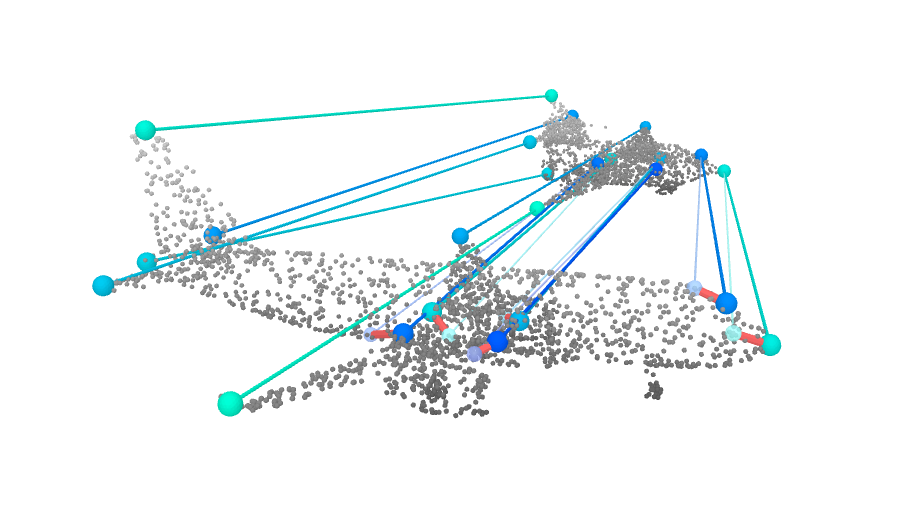
\includegraphics[width=\linewidth]{sup_mat/figures/airplane_top15_464a8718_x_dfa36bff_yaw-253p84_pitch76p57.png}
        \caption{Airplanes}
        \label{fig:example_a}
    \end{subfigure}
    \hfill
    \begin{subfigure}[b]{0.48\linewidth}
        \centering
        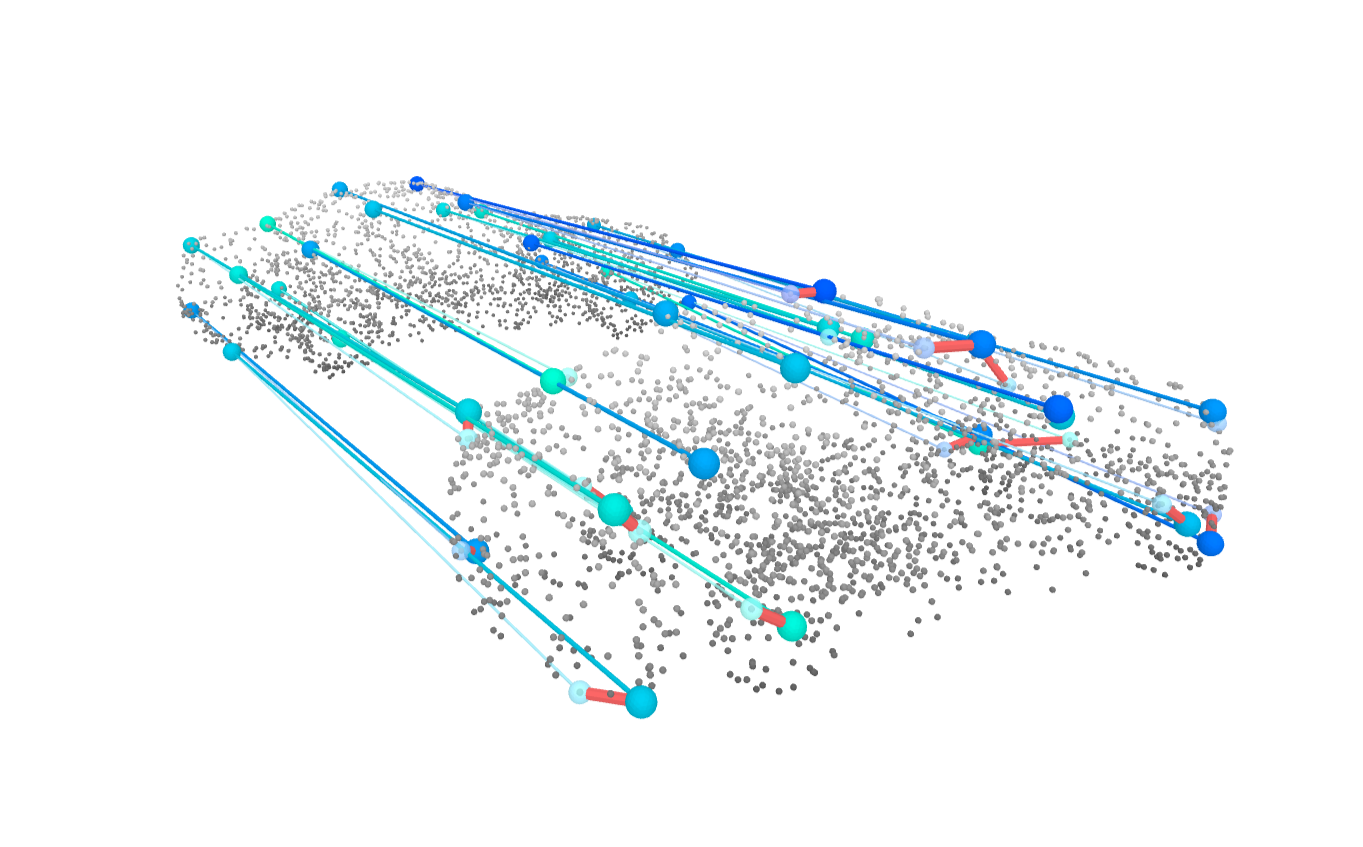
\includegraphics[width=\linewidth]{sup_mat/figures/car_top02_119033fe_x_1836f75b_yaw-298p07_pitch74p22.png}
        \caption{Cars}
        \label{fig:example_b}
    \end{subfigure}

    \caption{\textbf{Representative failure cases.}
We show examples of object pairs for which our predicted correspondences are close to the human-annotated keypoints, but still exhibit visible localization errors. Predicted correspondences are shown in lighter colors, while human annotations are shown in darker colors. Red lines connect each prediction to its corresponding ground-truth annotation, visualizing the error. These examples show that, although our pipeline usually identifies the correct semantic region, its predictions can be slightly displaced from the human labels.}
    \label{fig:two_images}
\end{figure}